
\let\negmedspace\undefined
\let\negthickspace\undefined
\documentclass[journal]{IEEEtran}
\usepackage[a5paper, margin=10mm, onecolumn]{geometry}
%\usepackage{lmodern} % Ensure lmodern is loaded for pdflatex
\usepackage{tfrupee} % Include tfrupee package

\setlength{\headheight}{1cm} % Set the height of the header box
\setlength{\headsep}{0mm}     % Set the distance between the header box and the top of the text

\usepackage{gvv-book}
\usepackage{gvv}
\usepackage{cite}
\usepackage{amsmath,amssymb,amsfonts,amsthm}
\usepackage{algorithmic}
\usepackage{graphicx}
\usepackage{textcomp}
\usepackage{xcolor}
\usepackage{txfonts}
\usepackage{listings}
\usepackage{enumitem}
\usepackage{mathtools}
\usepackage{gensymb}
\usepackage{comment}
\usepackage[breaklinks=true]{hyperref}
\usepackage{tkz-euclide} 
\usepackage{listings}
% \usepackage{gvv}                                        
\def\inputGnumericTable{}                                 
\usepackage[latin1]{inputenc}                                
\usepackage{color}                                            
\usepackage{array}                                            
\usepackage{longtable}                                       
\usepackage{calc}                                             
\usepackage{multirow}                                         
\usepackage{hhline}                                           
\usepackage{ifthen}                                           
\usepackage{lscape}
\begin{document}

\bibliographystyle{IEEEtran}
\vspace{3cm}

\title{4-4.2-9}
\author{AI24BTECH11005 - Bhukya Prajwal Naik
}
% \maketitle
% \newpage
% \bigskip
{\let\newpage\relax\maketitle}

\renewcommand{\thefigure}{\theenumi}
\renewcommand{\thetable}{\theenumi}
\setlength{\intextsep}{10pt} % Space between text and floats


\numberwithin{equation}{enumi}
\numberwithin{figure}{enumi}
\renewcommand{\thetable}{\theenumi}


\textbf{Question}:\\
 Find the directional and normal vectors of the following line: $x+y=4$.
\solution

\begin{table}[h!]
	\centering
	\begin{tabular}[12pt]{|c|c|c|}
    \hline
	\textbf{Information} & \textbf{Symbolic form} & \textbf{Value}\\ 
    \hline
	Given Line & $\vec{X} = \vec{h}+k\vec{m}$ & $x+y=6$\\
    \hline 
	Direction vector & $\vec{m}$ & \myvec{1 \\ -1}\\
    \hline
	Normal vector & $\vec{n}$ & \myvec{1 \\ 1}\\
    \hline   
    \end{tabular}

	\caption{Final Information}
	\label{4-4,2-9-tab-0}
\end{table}


The equation of the given line is:

\begin{align}
	4 &= x+y \\
	y &= 4-x \\
	\implies \myvec{x \\ y} &= \myvec{x \\ 4-x} =\myvec{0 \\ 4} +x\myvec{1 \\ -1} \\
	\vec{X} &= \vec{h} +k\vec{m}
\end{align}

Hence we get the direction vector:
\begin{align}
	\vec{m} &= \myvec{1 \\ -1}
\end{align}
then we get 
\begin{align}
	\vec{n} &= \myvec{1 \\ 1}
\end{align}


Hence, the direction vector of the line is given by $\vec{m} = \myvec{1 \\ -1}$ and the normal vector is $\vec{n} = \myvec{1 \\ 1}$.
\begin{figure}[h!]
	\centering
	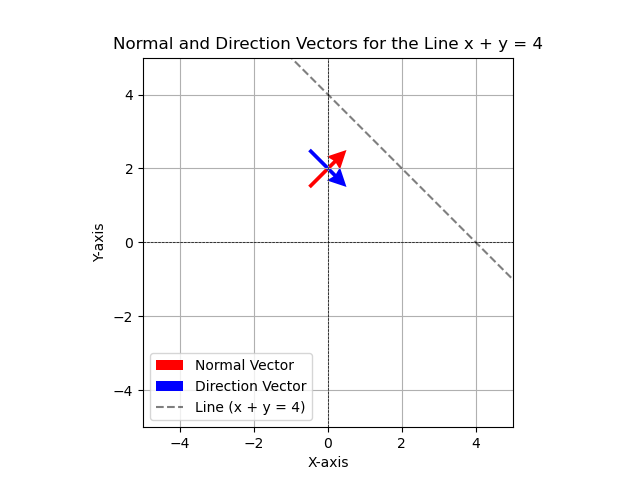
\includegraphics[width=0.7\textwidth]{Figure_1.png}
	\label{Graph}
	\caption{Lines and Vectors}
        \end{figure}




\end{document}
